\documentclass[pdflatex,compress,mathserif]{beamer}

%\usetheme[dark,framenumber,totalframenumber]{ElektroITK}
\usetheme[darktitle,framenumber,totalframenumber]{ElektroITK}

\usepackage[utf8]{inputenc}
\usepackage[T1]{fontenc}
\usepackage{lmodern}
\usepackage[bahasai]{babel}
\usepackage{amsmath}
\usepackage{amsfonts}
\usepackage{amssymb}
\usepackage{graphicx}
\usepackage{multicol}
\usepackage{extarrows}

\newcommand*{\Scale}[2][4]{\scalebox{#1}{$#2$}}%

\title{DIGITAL SIGNAL PROCESSING}
\subtitle{The Discrete Fourier Series}

\author{Mifta Nur Farid}

\begin{document}

\maketitle

\section{Introduction}

\begin{frame}
	\frametitle{Introduction}
	\begin{itemize}
		\item In Signal \& Systems:\\
		Fourier Transfrom (FT) \& z-Transfrom (z-T) $\rightarrow$ important analytic tools for representing discrete time signals \& systems.
		\item Convolution in time domain $\rightarrow$ multiplication in freq. domain in FT or in z domain in z-T.
		\item FT \& z-T are primary analytical tools but hard to implementing.
		\item FT is a function of a continuous variable $\omega$ $\rightarrow$ compute at infinite number of frequencies. $$ H(e^{j\omega}) = \sum\limits_{n=-\infty}^{+\infty} h(n)e^{-j \omega n} $$
	\end{itemize}
\end{frame}

\begin{frame}{Introduction}
	\begin{itemize}
		\item Another transform $\rightarrow$ the discrete Fourier trasform (DFT)
		\item Similar to FT and z-T, convolution $\rightarrow$ multiplication.
		\item Similar and also different properties to FT and z-T.
	\end{itemize}
\end{frame}

\section{The Discrete Fourier Series}

\begin{frame}
	\frametitle{The Discrete Fourier Series}
	\begin{center}
		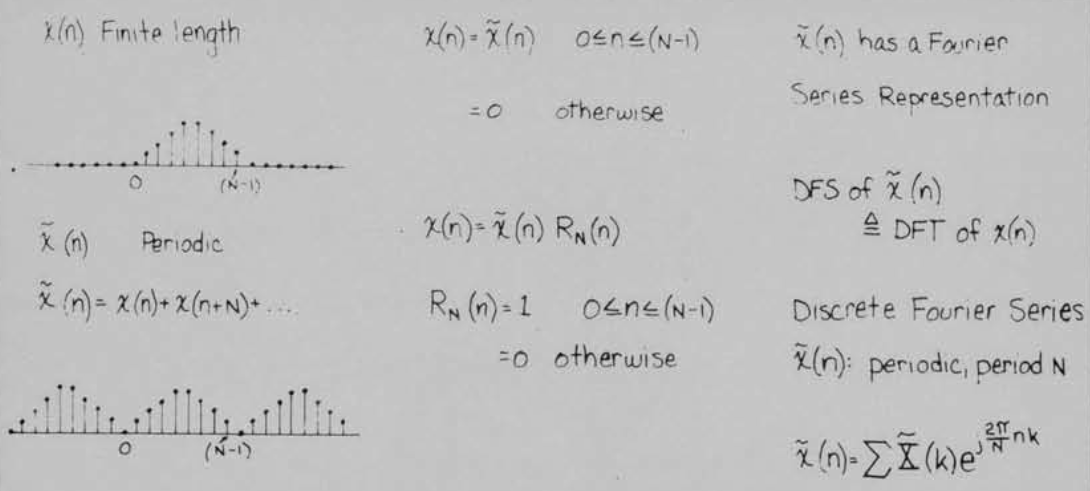
\includegraphics[width=\linewidth]{img/img01}
	\end{center}
\end{frame}

\begin{frame}{The Discrete Fourier Series}
	\begin{center}
		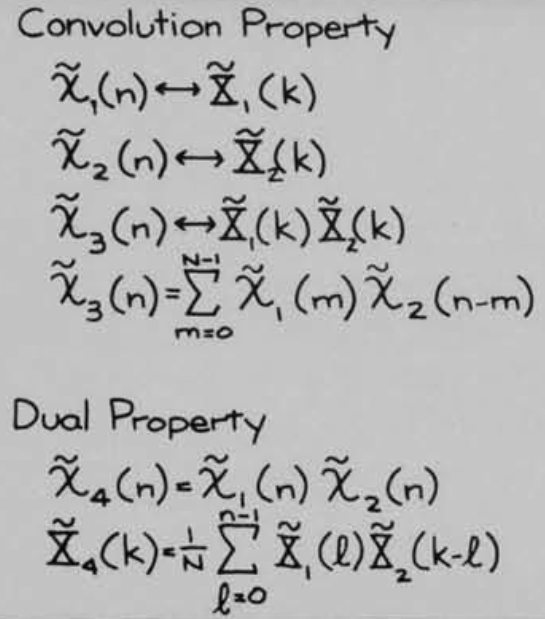
\includegraphics[width=0.5\linewidth]{img/img03}
	\end{center}
\end{frame}

\begin{frame}{The Discrete Fourier Series}
	\begin{center}
		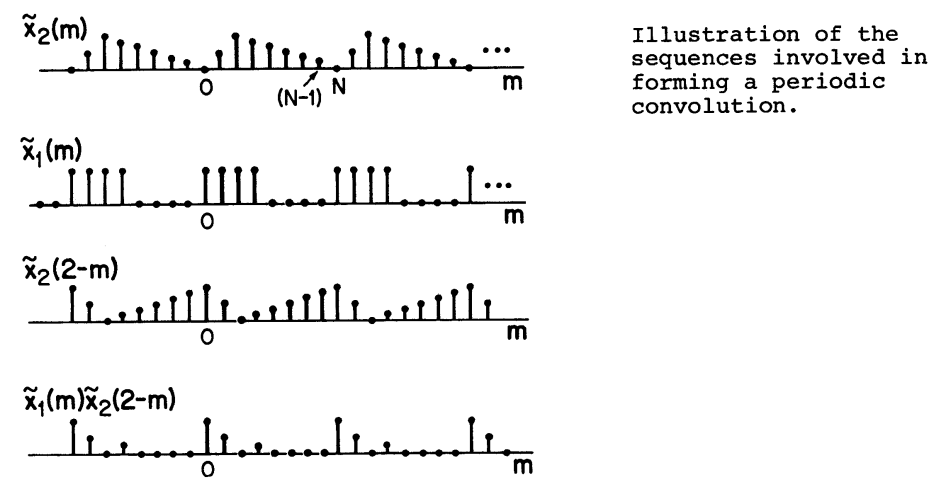
\includegraphics[width=\linewidth]{img/img04}
	\end{center}
\end{frame}

\begin{frame}
	\frametitle{Problems}
	\begin{center}
		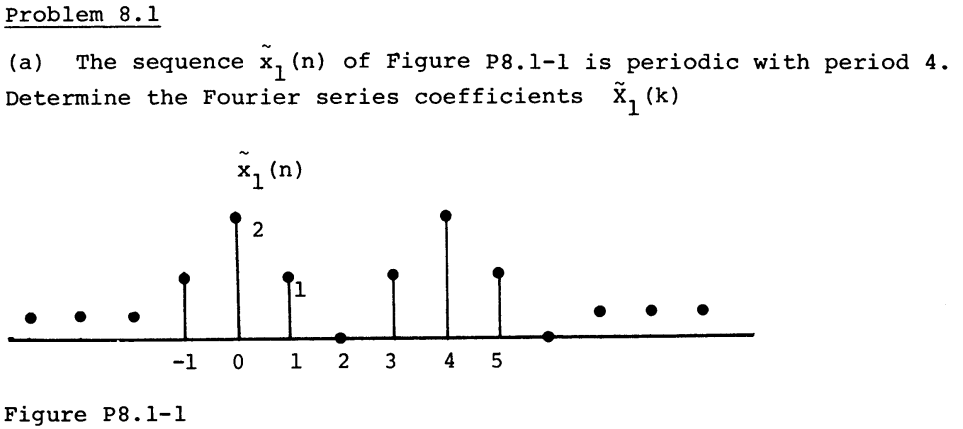
\includegraphics[width=\linewidth]{img/img05}
	\end{center}
\end{frame}

\begin{frame}{Problems}
	\begin{center}
		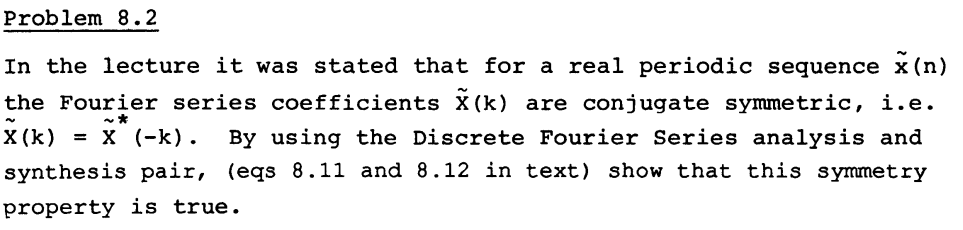
\includegraphics[width=\linewidth]{img/img06}
	\end{center}
\end{frame}

\begin{frame}{Problems}
	\begin{center}
		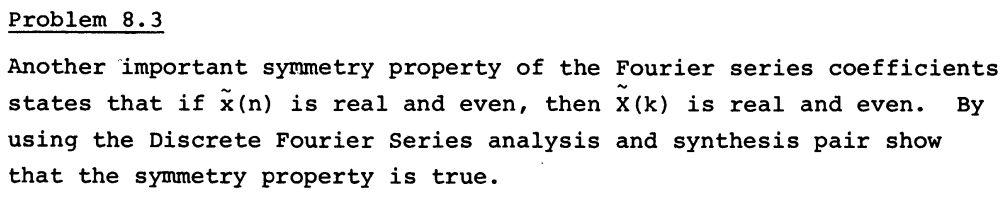
\includegraphics[width=\linewidth]{img/img07}
	\end{center}
\end{frame}

\begin{frame}{Problems}
	\begin{center}
		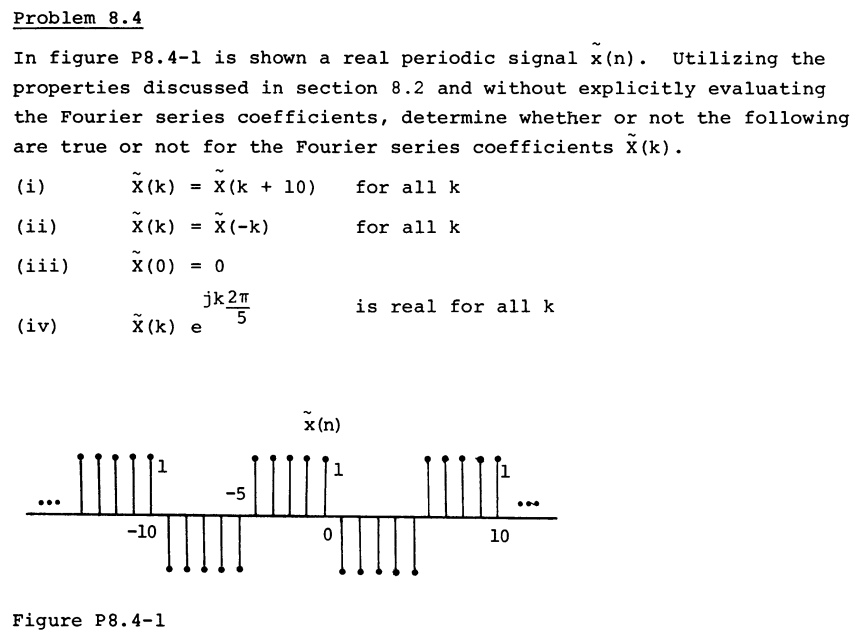
\includegraphics[width=0.9\linewidth]{img/img08}
	\end{center}
\end{frame}

\begin{frame}{Problems}
	\begin{center}
		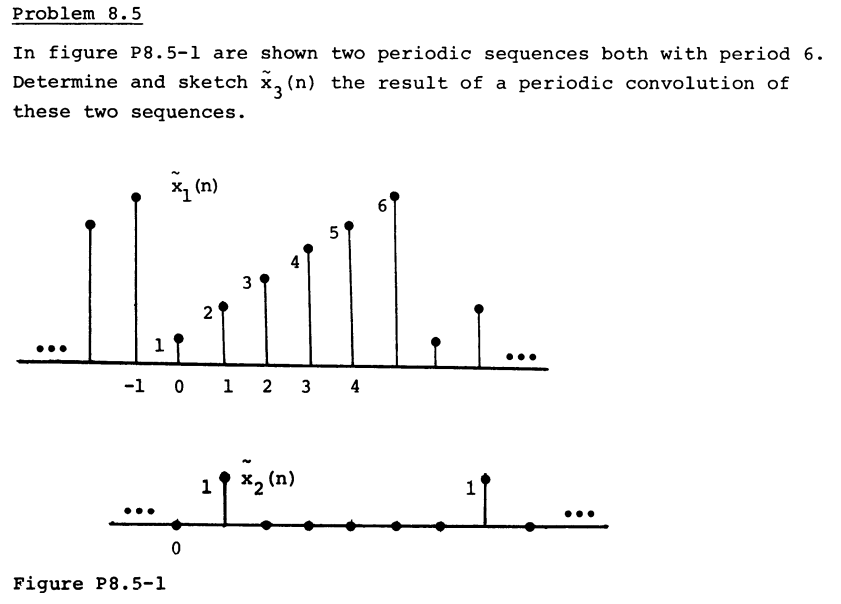
\includegraphics[width=0.9\linewidth]{img/img09}
	\end{center}
\end{frame}

\end{document}
